\documentclass{article}
\usepackage{geometry}
\usepackage{subcaption}
\usepackage{parskip}
\usepackage{graphicx}
\usepackage{pythonhighlight}
\usepackage{amsmath}
\newcommand{\code}[1]{\texttt{#1}}

\geometry{
  a4paper,
  margin=1in
}

\title{NLarge your dataset: Data augmentation for NLP}

\author{
  Ng Tze Kean \\
  \texttt{ngtzekean@gmail.com}
  \and
  Dexter Gui \\
  \texttt{dexter@email.com}
}

\begin{document}

\maketitle

\begin{abstract}

  In this report, we explore the application of data augmentation (DA) techniques
  for Natural Language Processing (NLP) using a variety of methods including
  Large Language Models (LLMs). We demonstrate the effectiveness of these
  techniques in enhancing the diversity and robustness of the training data,
  potentially improving the performance of NLP models. We present our
  methodology, experimental results, and discuss the implications of our
  findings.

  Overall, we found that use of statistical methods such as substitution for data
  augmentation has limited applications. The use of more advanced deep learning
  models such as RNN with attention mechanisms tend to perform better in this
  task. The best results were obtained using Large Language Models (LLMs) for DA,
  which significantly improved the performance of the model.

\end{abstract}

\section{Introduction}

DA is a widely used technique in machine learning to enhance the diversity and
robustness of training datasets. By artificially expanding the dataset, DA
helps improve the generalization capabilities of models, particularly in
scenarios where labeled data is scarce or expensive to obtain
\cite{DBLP:journals/corr/abs-2105-03075}. In the context of Natural Language
Processing (NLP), DA poses unique challenges due to the complexity and
variability of human language.

Traditional DA methods in NLP, such as synonym replacement, random insertion,
and back-translation, have shown limited effectiveness in generating diverse
and meaningful variations of text data. These methods often fail to capture the
nuanced semantics and contextual dependencies inherent in natural language,
leading to suboptimal improvements in model performance.

Recent advancements in deep learning, particularly the development of Large
Language Models (LLMs) like GPT-2, GPT-3, and T5, have opened new avenues for
DA in NLP. These models, pre-trained on vast corpora of text data, possess a
remarkable ability to generate coherent and contextually relevant text.
Leveraging LLMs for DA involves generating synthetic data samples by providing
prompts based on existing training examples.

\subsection{Literature Review}

DA has been a widely researched area in the field of Natural Language
Processing (NLP) due to its potential to enhance the diversity and robustness
of training datasets \cite{DBLP:journals/corr/abs-2105-03075}. In the context
of sentiment analysis, DA techniques are particularly valuable as they help
improve the generalization capabilities of models, especially when labeled data
is scarce \cite{li-specia-2019-improving}.

Rule based methods like random replacement are quick to implement but lack the
generalisability to different corpus. These methods aim to generate new
training samples by making small perturbations to the existing data, thereby
increasing the size of the training set and improving the generalization
capabilities of sentiment analysis models \cite{wei-zou-2019-eda}.

Interpolation methods such as synonym replacement has also been developed
\cite{sahin-steedman-2018-data} where words in a sentence are replaced with
their synonyms. This method has been shown to improve model performance by
introducing lexical diversity. However, it often fails to capture the nuanced
semantics and contextual dependencies inherent in natural language, leading to
suboptimal improvements in sentiment analysis tasks
\cite{sahin-steedman-2018-data}.

Leading us to the current state of the art, the use of LLMs for data
augmentation has shown promising results in improving the performance of NLP
models \cite{ding-etal-2024-data}. By leveraging the generative capabilities of
LLMs we are able to reduce the amount of noise introduced and thus generate a
higher quality dataset. Most of the research has been focused on NER tasks, and
we aim to explore the feasibility of using LLMs for DA in sentiment analysis
tasks to ascertain the effectiveness of this approach.

Our hypothesis is that the benefits of LLM DA will still continue to provide
superior performance in sentiment analysis tasks over pre-LLM DA methods.

\subsection{Objective}

In this project, we explore the application of DA techniques for sentiment
analysis in NLP. We aim to evaluate the effectiveness of traditional DA methods
such as random substitution and synonym replacement, as well as advanced
techniques using LLMs for data augmentation.

The outcome would be a python library made open source with the implemented
methods and algorithms for the community to use.

\subsection{Training and Evaluation}

To evaluate the performance gain of the DA techniques, we augmented the dataset
at different levels: 5\%, 10\%, and 20\%. Afterwards, we will attempt extreme
cases of DA at 50\%, 100\%, and 200\% to observe the trend of the performance.

The base line model will be trained on the original dataset using a Recurrent
Neural Network (RNN) model to perform sentiment classification on the
validation dataset. We will then retrain the model using the augmented dataset
and compare the performance metrics to assess the impact of DA on model
performance.

We will also include

\subsubsection{Model Architecture for Sentiment Classification}

The RNN model architecture consists of an embedding layer, followed by an RNN
layer, and a fully connected layer with a sigmoid activation function for
binary classification. The model was trained using the Adam optimizer with a
learning rate of \code{5e-4} and binary cross-entropy loss.

We adopted a pre-trained word embedding model to initialize the embedding layer
to transfer knowledge from the pre-trained model to our sentiment
classification task. The RNN layer uses a simple hidden layer our target is to
train that task layer to perform sentiment classification.

Our primary measure of improvement is the accuracy gain on the validation
dataset by the task specific RNN model. We also monitor the loss curves to
ensure that the model is not overfitting to the training data. Our hypothesis
is that the model will generalize better to unseen data with the augmented
dataset through various means to increase the volume of the corpus in
meaningful manners that will help the model learn and overfit less to the
training data.

\section{DA using Random Substitution}

In this subsection, we analyze the performance of DA using random substitution.

Let \( X = \{x_1, x_2, \ldots, x_n\} \) be a sequence of words in a text, where
\( x_i \) represents the \( i \)-th word in the sequence.

The random substitution process can be defined as follows:

For each word \( x_i \) in the sequence \( X \), with a probability \( p \),
swap \( x_i \) with its adjacent word if \( x_i \) is not a stop word. Where
\(x_j = x_{i+1}\) or \(x_j = x_{i-1}\).

\[
  x_i' =
  \begin{cases}
    \mathrm{swap}(x_i,x_j) & \mathrm{with\ probability\ } p   \\
    x_i                    & \mathrm{with probability } 1 - p
  \end{cases}
\]

where \( x_i' \) is the new word after substitution. The augmented sequence \(
X' = \{x_1', x_2', \ldots, x_n'\} \) is then used as the new training sample.

The random substitution process involves iterating over each word in the
sequence and swapping with a predefined probability \( p \). This introduces
variability into the dataset, potentially improving the robustness and
generalization capabilities of NLP models.

To evaluate the effectiveness of random substitution, we conducted experiments
with different levels of augmentation: 5\%, 10\%, and 20\% of the dataset. The
performance of the models trained with these augmented datasets was assessed
using accuracy score.

\subsection{Results and Analysis}

The results of our experiments indicate that the performance of the RNN model
keeps increasing with higher levels of augmentation. This suggests that data
augmentation provides a clear benefit for sentiment classification tasks.
Specifically, the model trained with 20\% augmented data achieved the highest
accuracy, followed by the models trained with 10\% and 5\% augmented data.
These findings highlight the importance of data augmentation in enhancing the
diversity and robustness of training datasets, leading to improved model
performance.

% insert image 
\begin{figure}[ht]
  \centering
  \begin{subfigure}[b]{0.3\textwidth}
    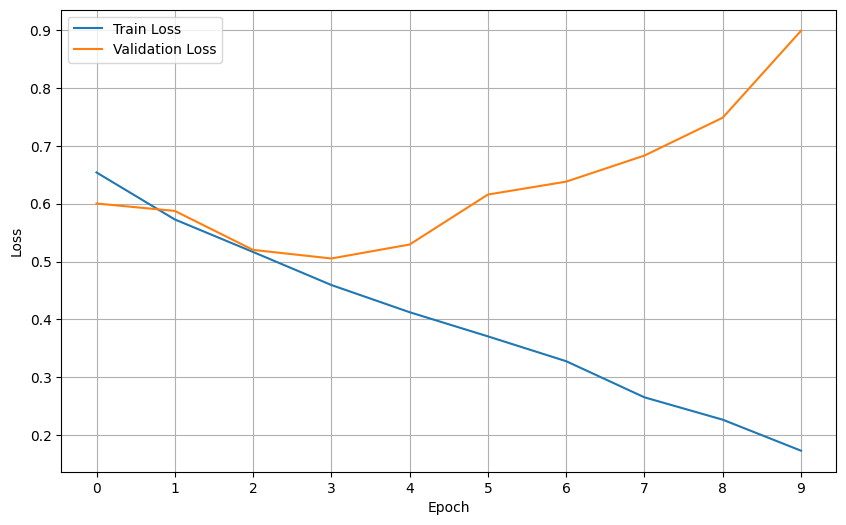
\includegraphics[width=\textwidth]{img/random_5.png}
    \caption{5\% Augmentation}
    \label{fig:random_5}
  \end{subfigure}
  \hfill
  \begin{subfigure}[b]{0.3\textwidth}
    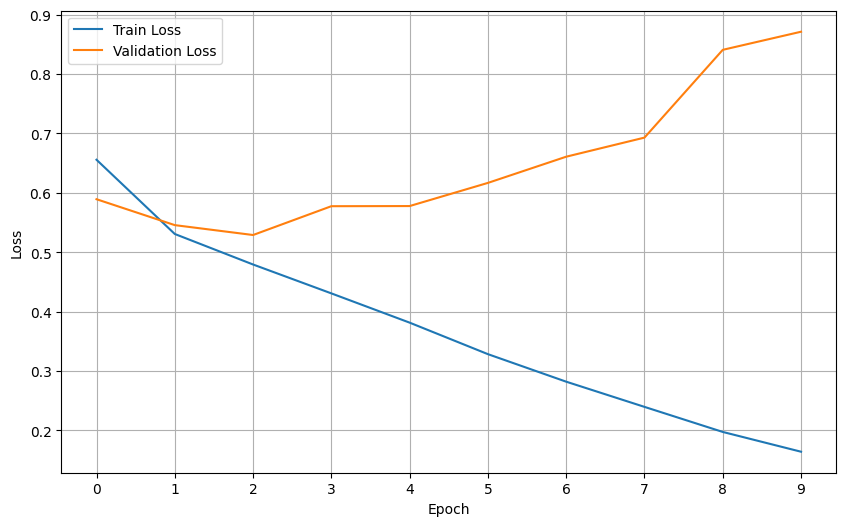
\includegraphics[width=\textwidth]{img/random_10.png}
    \caption{10\% Augmentation}
    \label{fig:random_10}
  \end{subfigure}
  \hfill
  \begin{subfigure}[b]{0.3\textwidth}
    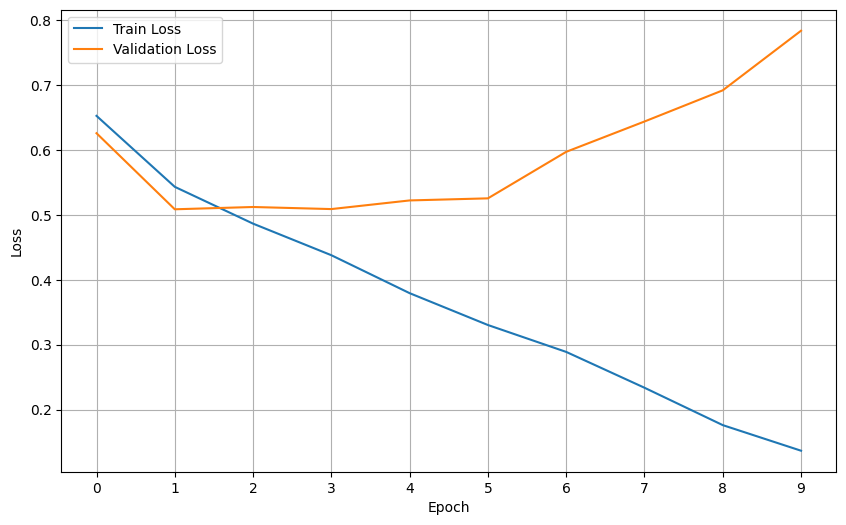
\includegraphics[width=\textwidth]{img/random_20.png}
    \caption{20\% Augmentation}
    \label{fig:random_20}
  \end{subfigure}
  \caption{Accuracy graphs for random substitution DA at 5\%, 10\%, and 20\% levels.}
  \label{fig:random_substitution_acc}
\end{figure}

The observed trend, where the performance of the RNN model improves with higher
levels of data augmentation, can be attributed to several key factors. Firstly,
data augmentation techniques like random substitution introduce increased data
diversity by exposing the model to a wider range of vocabulary and sentence
structures. This diversity helps the model learn more robust representations,
enhancing its ability to generalize to unseen examples. Secondly, data
augmentation mitigates overfitting by effectively increasing the size of the
training dataset, reducing the likelihood of the model memorizing specific
examples and encouraging it to learn general patterns instead. Additionally,
the introduction of variations in the training data makes the model more robust
to noise and variations in real-world input data. This robustness is crucial
for achieving good performance on unseen data. Furthermore, data augmentation
acts as a form of regularization, preventing the model from becoming too
complex and overfitting the training data. By providing a more comprehensive
training dataset, data augmentation improves the model's generalization
capabilities, leading to better performance on validation and test datasets.
Collectively, these factors contribute to the model's enhanced ability to learn
effectively from the training data and perform better on unseen examples.

\section{DA using Synonym Substitution}

In this subsection, we explore the performance of DA using synonym
substitution.

Let \( X = \{x_1, x_2, \ldots, x_n\} \) be a sequence of words in a text, where
\( x_i \) represents the \( i \)-th word in the sequence. Let \( S(x_i) \) be
the set of synonyms for the word \( x_i \).

The synonym substitution process can be defined as follows:

For each word \( x_i \) in the sequence \( X \), with a probability \( p \),
replace \( x_i \) with a randomly chosen synonym from \( S(x_i) \).
Mathematically, this can be expressed as:

\[
  x_i' =
  \begin{cases}
    \text{random}(S(x_i)) & \text{with probability } p     \\
    x_i                   & \text{with probability } 1 - p
  \end{cases}
\]

where \( x_i' \) is the new word after substitution, and
\(\text{random}(S(x_i))\) denotes a randomly selected synonym from the set \(
S(x_i) \).

The augmented sequence \( X' = \{x_1', x_2', \ldots, x_n'\} \) is then used as
the new training sample.

\subsection{Results and Analysis}

We can see from the results that generally as the augmentation level increases,
the performance of the model steadily increases as well.

% insert image 
\begin{figure}[ht]
  \centering
  \begin{subfigure}[b]{0.3\textwidth}
    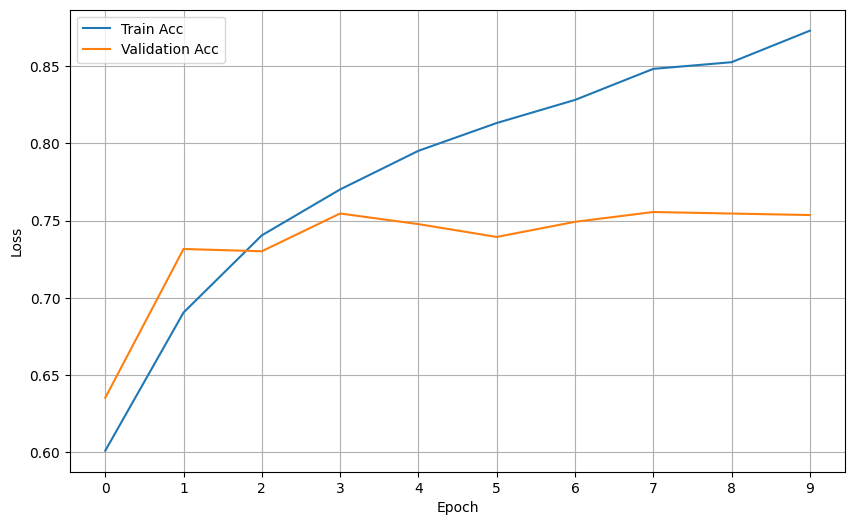
\includegraphics[width=\textwidth]{img/synonym_5.png}
    \caption{5\% Augmentation}
    \label{fig:synonym_5}
  \end{subfigure}
  \hfill
  \begin{subfigure}[b]{0.3\textwidth}
    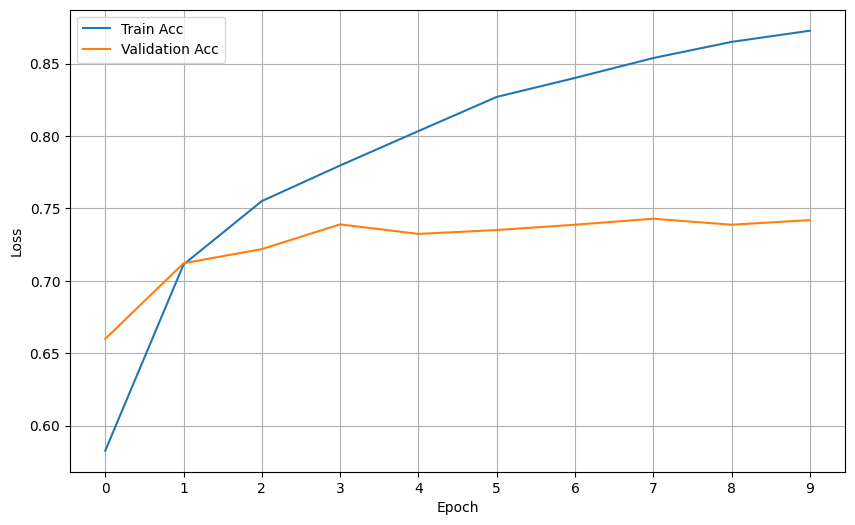
\includegraphics[width=\textwidth]{img/synonym_10.png}
    \caption{10\% Augmentation}
    \label{fig:synonym_10}
  \end{subfigure}
  \hfill
  \begin{subfigure}[b]{0.3\textwidth}
    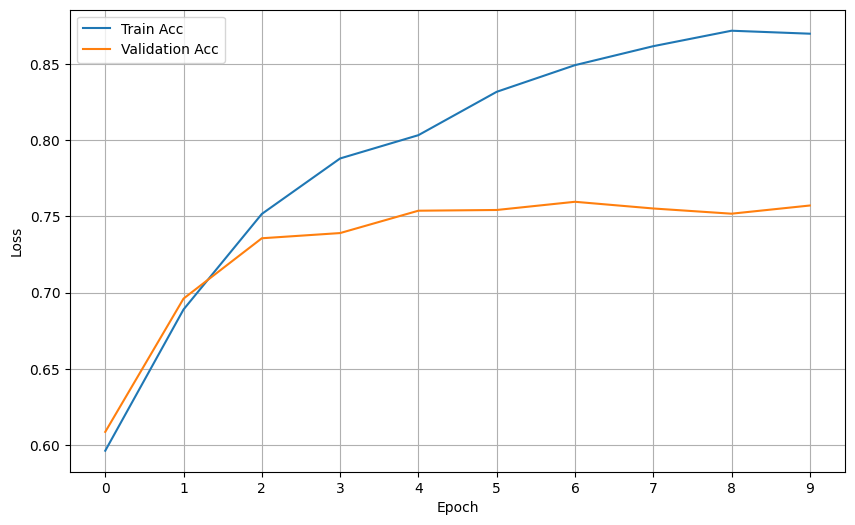
\includegraphics[width=\textwidth]{img/synonym_20.png}
    \caption{20\% Augmentation}
    \label{fig:synonym_20}
  \end{subfigure}
  \caption{Accuracy graphs for synonym substitution DA at 5\%, 10\%, and 20\% levels.}
  \label{fig:synonym_substitution_acc}
\end{figure}

\section{Extreme DA}

We define extreme DA as augmentation past 50\% of the dataset. To explore the
trend of the performance, we augmented the dataset at 50\%, 100\% and 200\%
levels on each of the above methods and observed the performance of the model.

\subsection{Results and Analysis}

What is interesting is the continued improvement of the model. The RNN model
consistently improves with higher levels of augmentation, while the LSTM model
is sporadic and shows instability. This suggests that the RNN model is more
robust to the increased data diversity introduced by extreme DA, while the LSTM
model may struggle to learn effectively from the augmented data.

\begin{figure}[ht]
  \centering
  \begin{subfigure}[b]{0.3\textwidth}
    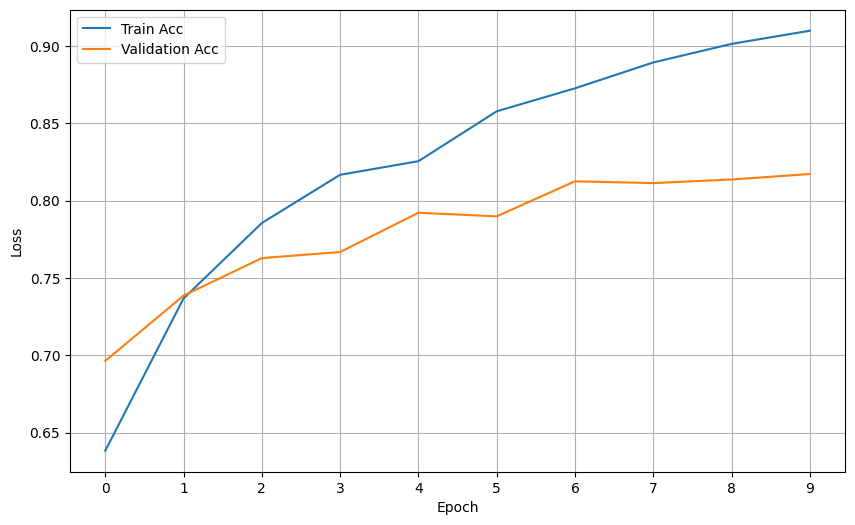
\includegraphics[width=\textwidth]{img/random_50.png}
    \caption{50\% Augmentation}
    \label{fig:random_50}
  \end{subfigure}
  \hfill
  \begin{subfigure}[b]{0.3\textwidth}
    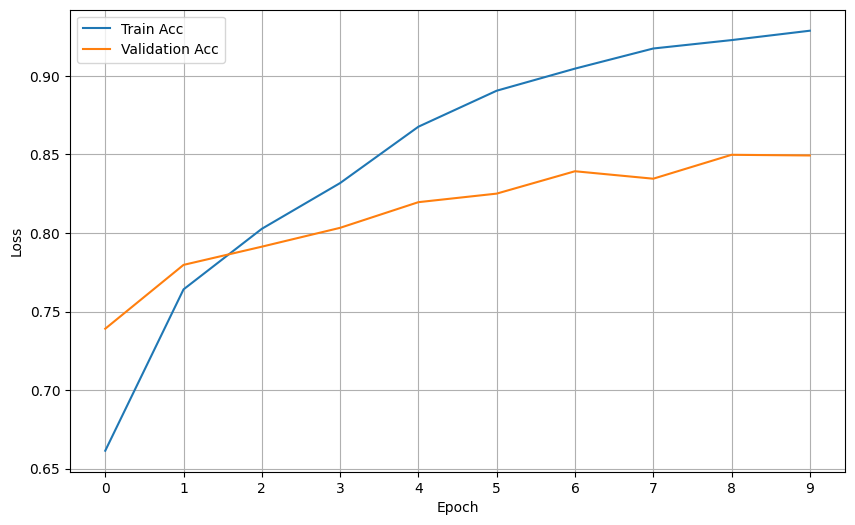
\includegraphics[width=\textwidth]{img/random_100.png}
    \caption{100\% Augmentation}
    \label{fig:random_100}
  \end{subfigure}
  \hfill
  \begin{subfigure}[b]{0.3\textwidth}
    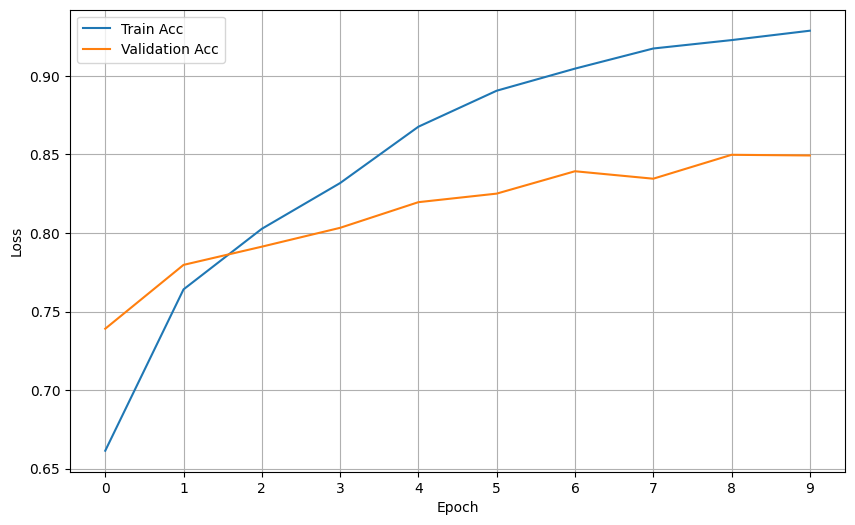
\includegraphics[width=\textwidth]{img/random_100.png}
    \caption{200\% Augmentation}
    \label{fig:random_100}
  \end{subfigure}
  \caption{Accuracy graphs for random substitution DA at 50\%, 100\%, and 200\% levels.}
  \label{fig:random_extreme_substitution_acc}
\end{figure}

\begin{figure}[ht]
  \centering
  \begin{subfigure}[b]{0.3\textwidth}
    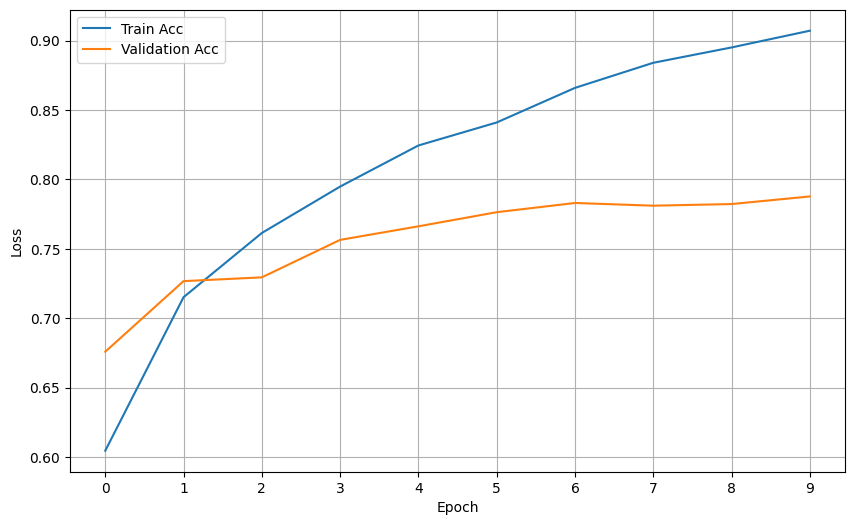
\includegraphics[width=\textwidth]{img/synonym_50.png}
    \caption{50\% Augmentation}
    \label{fig:synonym_50}
  \end{subfigure}
  \hfill
  \begin{subfigure}[b]{0.3\textwidth}
    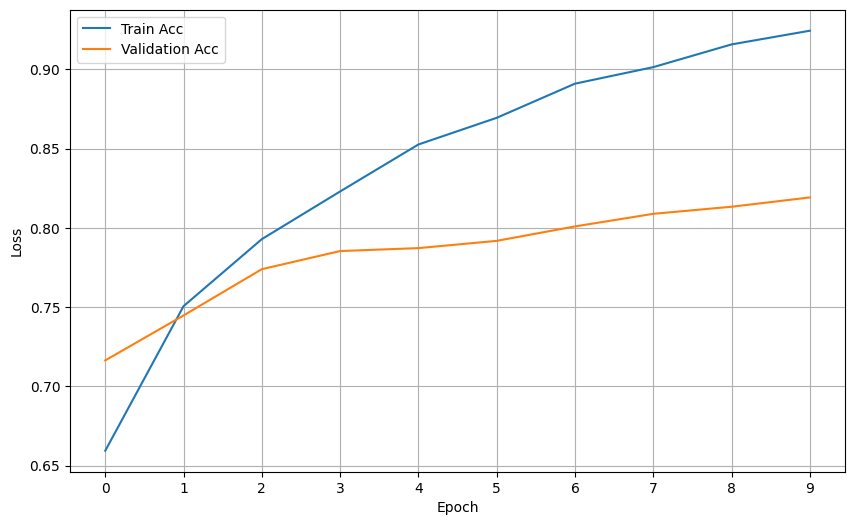
\includegraphics[width=\textwidth]{img/synonym_100.png}
    \caption{100\% Augmentation}
    \label{fig:synonym_100}
  \end{subfigure}
  \hfill
  \begin{subfigure}[b]{0.3\textwidth}
    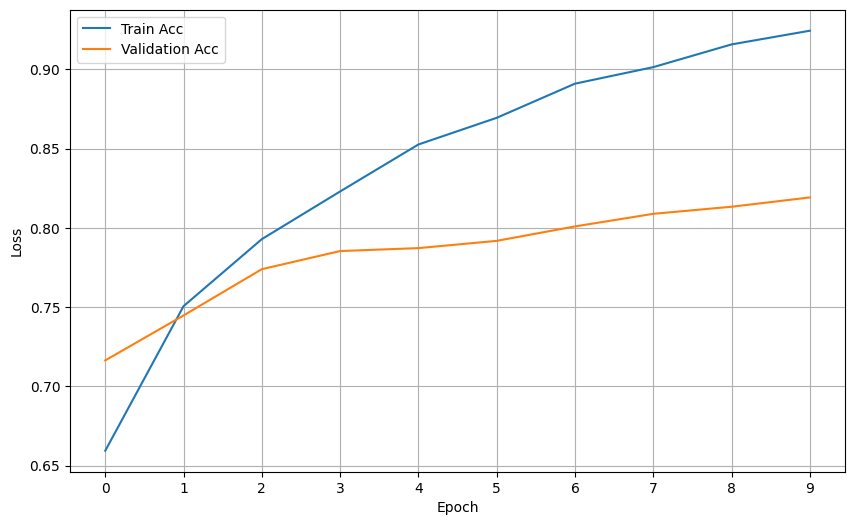
\includegraphics[width=\textwidth]{img/synonym_100.png}
    \caption{200\% Augmentation}
    \label{fig:synonym_100}
  \end{subfigure}
  \caption{Accuracy graphs for synonym substitution DA at 50\%, 100\%, and 200\% levels.}
  \label{fig:synonym_extreme_substitution_acc}
\end{figure}

\section{DA using Hybrid (Synonym + Random) Substitution}

In light of the results from above, we are interested how the performance might
continue to scale

\begin{figure}[ht]
  \centering
  \begin{subfigure}[b]{0.45\textwidth}
    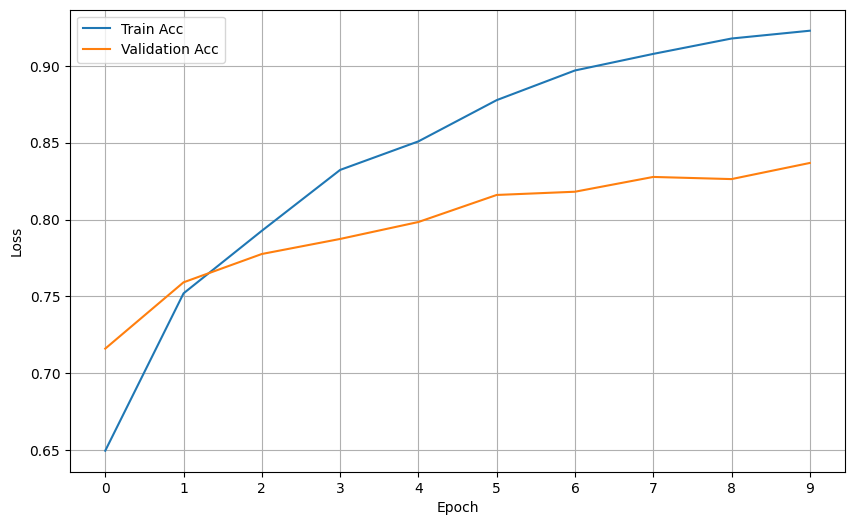
\includegraphics[width=\textwidth]{img/hybrid_100_rnn.png}
    \caption{50\% Random + 50\% Synonym Augmentation on RNN}
    \label{fig:hybrid_100_rnn}
  \end{subfigure}
  \hfill
  \begin{subfigure}[b]{0.45\textwidth}
    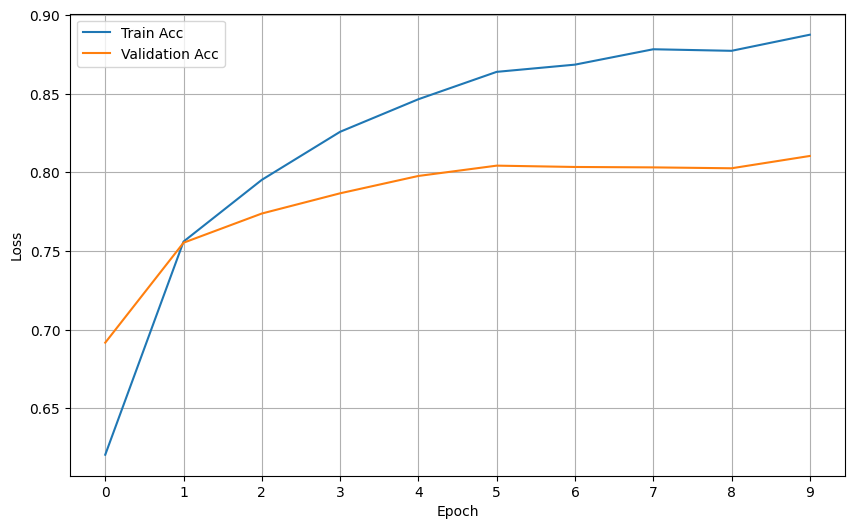
\includegraphics[width=\textwidth]{img/hybrid_100_lstm.png}
    \caption{50\% Random + 50\% Synonym Augmentation on LSTM}
    \label{fig:hybrid_100_lstm}
  \end{subfigure}
  \caption{Accuracy graphs for synonym substitution DA at 50\%, 100\%, and 200\% levels.}
  \label{fig:hybrid_extreme_substitution_acc}
\end{figure}

\section{DA using LLMs}

To enhance the diversity and robustness of our dataset, we employed a data
augmentation technique leveraging pre-trained Large Language Models (LLM) from
the Transformers library.

Specifically, we utilized the model to generate synthetic data samples by
providing prompts based on existing training examples. By carefully controlling
the generation parameters, we were able to produce high-quality, diverse, and
relevant augmented samples that expanded the scope of our training data,
potentially improving model generalization and performance.

\subsubsection{LLM selection}

We would like to note some of the challenges of selection of the LLM model for
DA. The choice of the model is crucial as it determines the quality of the
generated samples. We experimented with several models, including GPT-2, GPT-3,
and T5. As we tried to perform prompt engineering to generate diverse samples,
we found that these models could not adequately paraphrase the training data,
more often than not, producing the exact same text or slightly modified
versions of the original text.

We suspect that these LLM do not perform well due to the lack of contextual
information in the prompt. We hypothesize that the models require more
contextual information to generate diverse samples. We realised that a model
that allows us to specify a role for the prompt, we would be able to generate
more diverse samples.

\subsubsection{Prompt Engineering}

We proceeded to experiment with the Qwen model, with some of the techniques
applied from \cite{promptingguide}. We found that the Qwen model allows us to
specify a role for the prompt, which allows us to instruct the model to
specifically only paraphrase the verbs and structure of the sentence. This
allows us to generate a text that differs from the original text, while still
retaining the meaning of the original text.

\subsubsection{Results and Analysis}

We observed that with the Qwen model, we were able to generate diverse and
relevant samples, yet the performance of the model did not improve and in fact
there was significant degradation in the performance of the model. This can be
seen from Figure \ref{fig:llm_substitution_loss} and Table
\ref{table:rnn_performance}. This is very unexpected as we hypothesized that
the diverse samples would improve the performance of the model. Our hypothesis
that using a expert model to increase the diversity of the samples would
improve the performance of the model was not supported by the results.

\begin{figure}[ht]
  \centering
  \begin{subfigure}[b]{0.3\textwidth}
    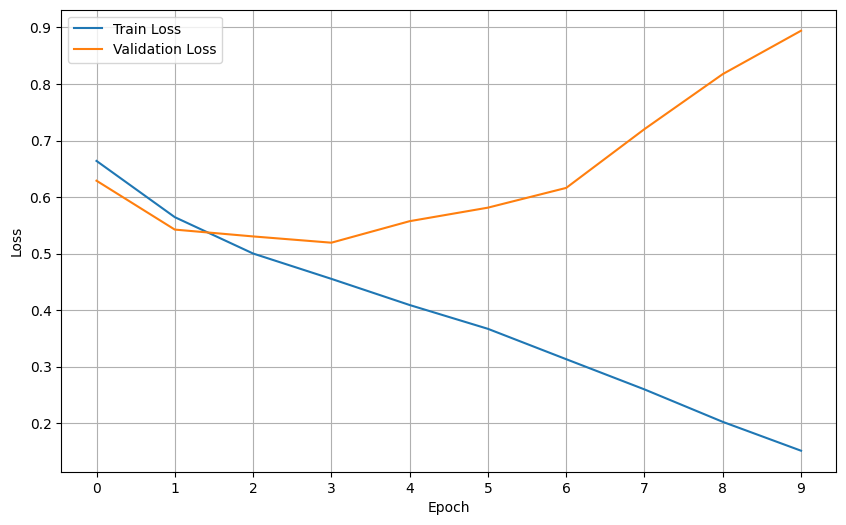
\includegraphics[width=\textwidth]{img/llm_loss_5.png}
    \caption{5\% Augmentation}
    \label{fig:llm_loss_5}
  \end{subfigure}
  \hfill
  \begin{subfigure}[b]{0.3\textwidth}
    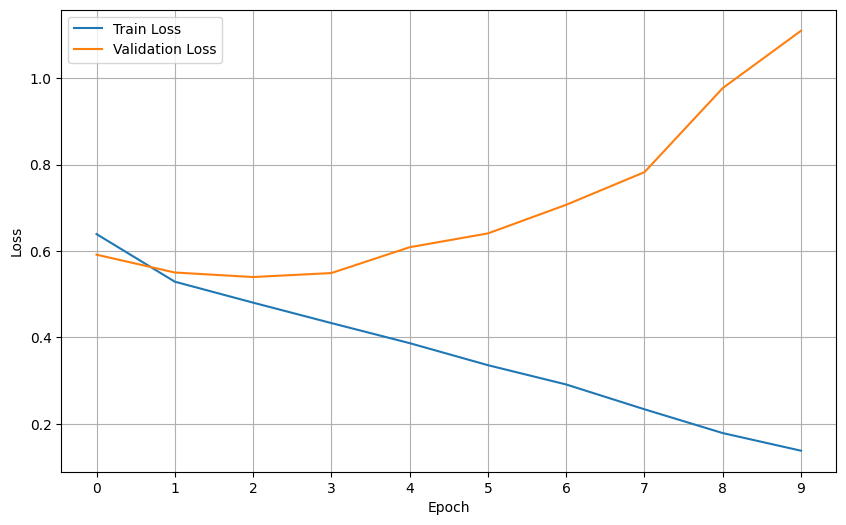
\includegraphics[width=\textwidth]{img/llm_loss_10.png}
    \caption{10\% Augmentation}
    \label{fig:llm_loss_10}
  \end{subfigure}
  \hfill
  \begin{subfigure}[b]{0.3\textwidth}
    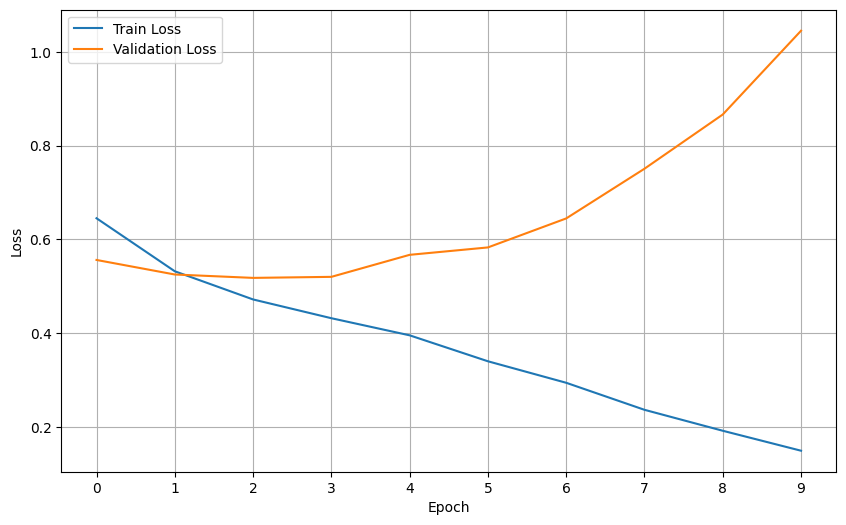
\includegraphics[width=\textwidth]{img/llm_loss_20.png}
    \caption{20\% Augmentation}
    \label{fig:llm_loss_20}
  \end{subfigure}
  \caption{Loss graphs for llm substitution DA at 5\%, 10\%, and 20\% levels.}
  \label{fig:llm_substitution_loss}
\end{figure}

We examined the possible causes of this unexpected result and found that the
augmentation generated by the Qwen model was too long that the RNN suffered
from vanishing gradients. We hypothesize that there was 2 main issues.
% bullet points with numbers
\begin{enumerate}
  \item Vanishing gradients due to the long sequences generated
  \item RNN suffering from the long sequences generated
\end{enumerate}

\begin{table}[ht]
  \centering
  \begin{tabular}{|c|c|c|}
    \hline
    \textbf{Augmentation Level} & \textbf{Train Accuracy} & \textbf{Validation Accuracy} \\
    \hline
    5\%                         & 0.947                   & 0.717                        \\
    \hline
    10\%                        & 0.950                   & 0.697                        \\
    \hline
    20\%                        & 0.945                   & 0.695                        \\
    \hline
  \end{tabular}
  \caption{Performance of RNN model with different levels of DA with 100 token per sample limit.}
  \label{table:rnn_performance}
\end{table}

We tailored our approach in 2 ways: we limited the token length of the
generated samples to 20 tokens and we changed the RNN model to a Long
Short-Term Memory (LSTM) model to better handle the long sequences. We found
that the performance of the model improved significantly, and the model was
able to learn and generalize better.

\section{NLarge: A Python Library for Data Augmentation}

We developed a Python library called NLarge to DA for NLP sentiment analysis.
The library provides the methods and functions used in this report along with
models that can be used for sentiment analysis. The goal is to provide a
toolkit where users can easily experiment with different DA techniques at
various levels and models for sentiment analysis tasks.

We also made a website to provide end users with some information
\code{https://nlarge.com} such that we have an end to end solution for users to
use.


\section{Discussion}

We find it interesting that the use of statistical methods still has a place in
the field of DA in post LLM era. The use of LLMs for DA has shown promising
results in improving the performance of NLP models. While the use of LLMs for
DA produces schematically diverse samples with better quality, the computation
cost is high especially if the augmentation level is high.

\section{Conclusion}
% Summarize your findings and future work

\bibliographystyle{plain}
\bibliography{bibliography.bib}

\end{document}